\documentclass{beamer}
\usetheme{Boadilla}
\usepackage[utf8]{inputenc}
\usepackage{graphicx}
\graphicspath{ {./images/} }
\usepackage{hyperref}

\title{Git Tutorial}
\author{Augusto Fraga Giachero}
\date{\today}

\AtBeginSection[]{
  \begin{frame}
  \vfill
  \centering
  \begin{beamercolorbox}[sep=8pt,center,shadow=true,rounded=true]{title}
    \usebeamerfont{title}\insertsectionhead\par
  \end{beamercolorbox}
  \vfill
  \end{frame}
}

\begin{document}

% Title page frame
\begin{frame}
  \titlepage
\end{frame}

% Outline frame
\begin{frame}{Outline}
  \tableofcontents
\end{frame}

\section{Basics}

\subsection{Configuration}
\begin{frame}{Configuration}
  \begin{itemize}
    \item Before using Git, it is a good idea to set some global configurations:
  \end{itemize}
  \begin{block}{}
    \texttt{\$ git config --global user.name "Augusto Fraga Giachero"} \\
    \texttt{\$ git config --global user.email augusto.fraga@lnls.br} \\
    \texttt{\$ git config --global pull.rebase true} or \texttt{false} \\
    \texttt{\$ git config --global core.editor vim}
  \end{block}
  \begin{flushright}
    Note: The email used here has nothing to do \\ with Gitlab/Github/Bitbucket credentials.
  \end{flushright}
\end{frame}

\subsection{Creating a Repository}
\begin{frame}{Creating a Repository}
  \begin{itemize}
    \item You should initialize a git repository in the root directory of the project, it doesn't need to be empty;
    \item It is a good idea to also include a \texttt{.gitignore} file from the beginning to avoid accidentally commiting temporary files or files not relevant to the project. You can use third party tools to automatically generate \texttt{.gitignore} files like \href{https://github.com/simonwhitaker/gibo}{gibo} or \href{https://www.toptal.com/developers/gitignore/}{gitignore.io}.
  \end{itemize}
  \begin{block}{}
    \texttt{\$ mkdir project \&\& cd project} \\
    \texttt{\$ git init} \\
    \texttt{\$ gibo dump vim emacs linux windows macos > .gitignore}
  \end{block}
\end{frame}

\subsection{Staging}
\begin{frame}{Staging}
  \begin{itemize}
    \item Before commiting, you should stage your modifications;
    \item Avoid using \texttt{git add .} as it may inadvertently stage undesirable files. \texttt{git add --update} will only add files which are already tracked by git, which is usually closer to the desired effect;
    \item You can stage parts of a file with \texttt{git add -p} \textit{file};
    \item To unstage a file, use the \texttt{git reset} \textit{file} command.
  \end{itemize}
  \begin{block}{}
    \texttt{\$ git add .gitignore} \\
    \texttt{\$ git diff --staged}
  \end{block}
\end{frame}

\subsection{Commiting}
\begin{frame}{Commiting}
  \begin{itemize}
    \item After staging your modifications, its time to commit the changes;
    \item Commit messages ideally should contain a title, following a blank line, and a more in-depth explanation of the changes;
    \item A commit should cover a single `scope', avoid grouping unrelated changes in a single commit.
  \end{itemize}
  \begin{block}{}
    \texttt{\$ git commit}
  \end{block}
  \begin{scriptsize}
    \begin{verbatim}
commit 144523468ee1b155135756dfdb3a14bda6382ab8
Author: Augusto Fraga Giachero <augusto.fraga@lnls.br>
Date:   Fri Nov 1 14:17:47 2024 -0300

    Include .gitignore file
    
    Ignore temporary files of major platforms and text editors. Generated
    with gibo [1].
    
    [1]: https://github.com/simonwhitaker/gibo
\end{verbatim}

  \end{scriptsize}
\end{frame}

\subsection{Branching}
\begin{frame}{Branching}
  \begin{itemize}
    \item Branches are very useful when implementing new features or testing new ideas without interfering with the main development history;
    \item Can also be used to maintain older versions of a project in parallel with newer versions;
    \item Essential part of the code review process.
  \end{itemize}
  \begin{block}{}
    \texttt{\$ git switch -c new-branch} \\
    \texttt{\$ echo "\# Nice documentation" > README.md} \\
    \texttt{\$ git add README.md} \\
    \texttt{\$ git commit}
  \end{block}
\end{frame}

\subsection{Merging}
\begin{frame}{Merging}
  \begin{itemize}
    \item After the work is done in the `feature' branch, it can be merged back to the `master'/`main'/`devel' branch;
    \item There are different merge strategies:
    \begin{itemize}
      \item `True' merge;
      \item Fast forward merge;
      \item Squash merge;
      \item Rebase merge.
    \end{itemize}
  \end{itemize}
  \begin{block}{}
    \texttt{\$ git switch master} \\
    \texttt{\$ git merge new-branch}
  \end{block}
\end{frame}

\begin{frame}{True Merges}
  \begin{itemize}
    \item Will create a new `merge' commit that references two or more parent commits;
    \item Any conflicts will be solved in the merge commit, preserving the original history in the source branch;
    \item The history is a bit more complicated to follow, as the branch now contains a `directed acyclic graph' instead of a single `thread' of commits.
  \end{itemize}
  \begin{center}
    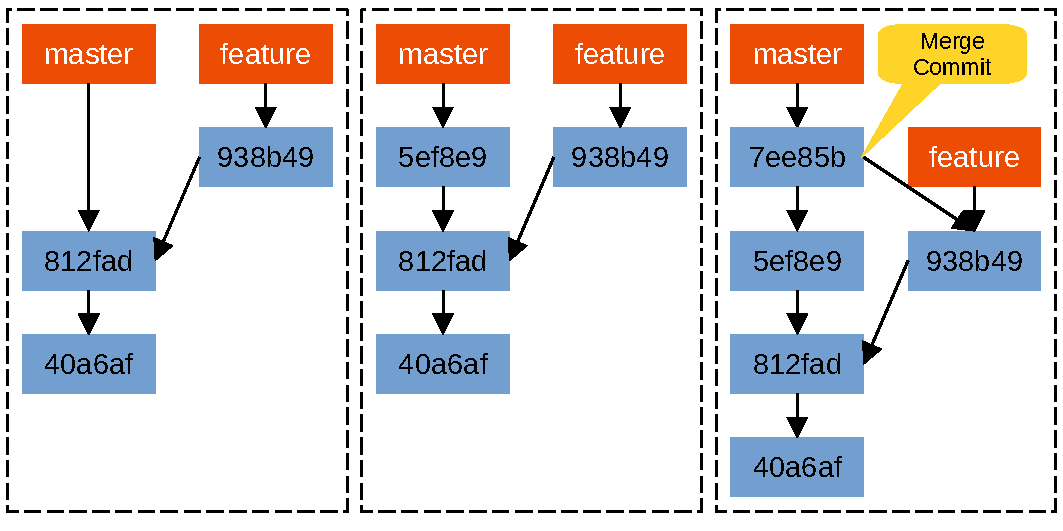
\includegraphics[scale=0.5]{git-true-merge}
  \end{center}
\end{frame}

\begin{frame}{Fast Forward Merges}
  \begin{itemize}
    \item Only possible if the destination branch doesn't have commits that aren't in the source branch, i.e. the source branch's history includes the top of the destination branch;
    \item Doesn't create new commits, just updates the branch pointer;
    \item It is the default behavior of \texttt{git merge} if it is possible, otherwise a true merge will be done.
  \end{itemize}
  \begin{center}
    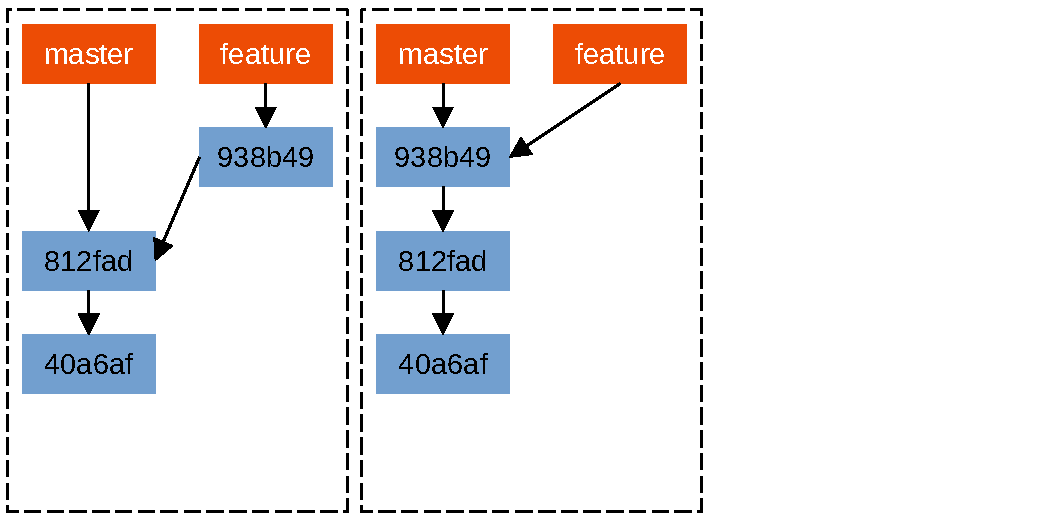
\includegraphics[scale=0.5]{git-fast-forward-merge}
  \end{center}
\end{frame}

\begin{frame}{Squash Merges}
  \begin{itemize}
    \item Takes the new commits in the source branch and 'squashes' into a single commit in the destination branch;
    \item Doesn't preserve the history of the source branch in the destination branch.
  \end{itemize}
  \begin{center}
    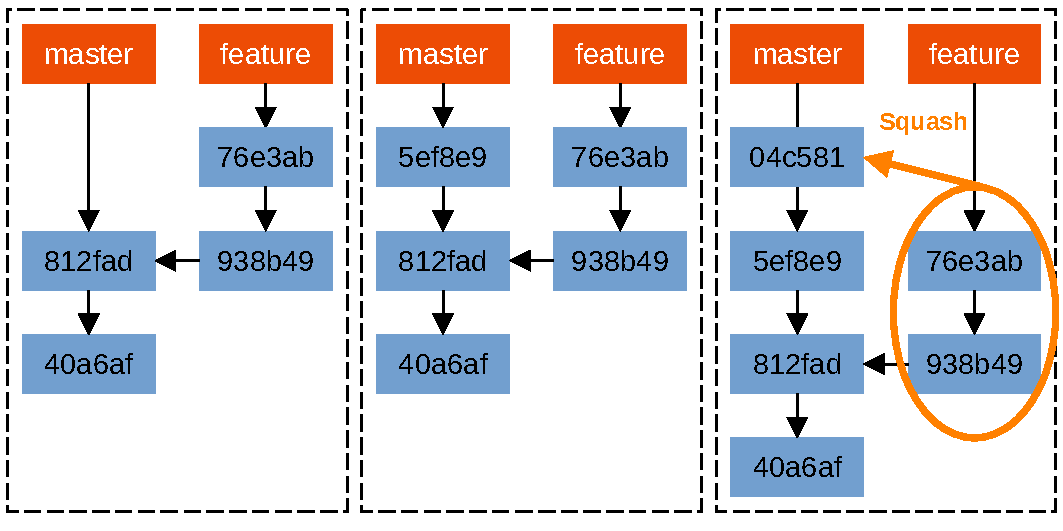
\includegraphics[scale=0.5]{git-squash-merge}
  \end{center}
\end{frame}

\begin{frame}{Rebase Merges}
  \begin{itemize}
    \item Re-applies the new commits in the source branch to the top of the destination branch;
    \item Re-writes the history of the source branch, so it must be used with care to avoid changing the history of public development branches;
    \item Keeps the history `linear' (i.e. no merge commits pointing to two or more commits).
  \end{itemize}
  \begin{center}
    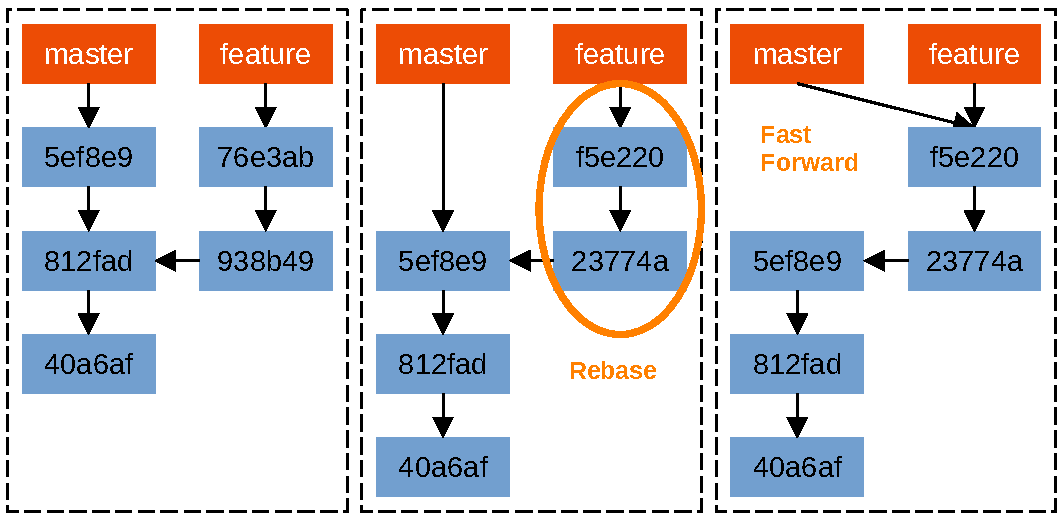
\includegraphics[scale=0.5]{git-rebase-merge}
  \end{center}
\end{frame}

\subsection{Merge conflicts}
\begin{frame}{Merge conflicts}
  \begin{itemize}
    \item If the same file is modified in different branches that have diverged, merging these branches will often lead to conflicts;
    \item It is only possible to merge text files, with binary files you have to choose between either branch;
    \item Solving conflicts requires manual intervention.
  \end{itemize}
  \begin{block}{}
    \texttt{\$ echo "Be nice to others when asking for help." >> README.md} \\
    \texttt{\$ git commit} \\
    \texttt{\$ git switch new-branch} \\
    \texttt{\$ echo "Remember to turn on your computer before using this." >> README.md} \\
    \texttt{\$ git commit} \\
    \texttt{\$ git switch master} \\
    \texttt{\$ git merge new-branch}
  \end{block}
\end{frame}

\subsection{Tagging}
\begin{frame}{Tagging}
  \begin{itemize}
    \item A friendly name to a specific commit;
    \item Frozen in time, i.e. you can't add commits to a tag;
    \item Commonly used to refer to release versions of a project.
  \end{itemize}
  \begin{block}{}
    \texttt{\$ git tag v0.0.1}
  \end{block}
\end{frame}

\subsection{Stashing}
\begin{frame}{Stashing}
  \begin{itemize}
    \item Sometimes when you have done some work, but it isn't ready to commit, and you want to change branches quickly, you will need to `stash' the changes;
    \item It basically saves your current un-commited work in the stash stack for later use.
  \end{itemize}
  \begin{block}{}
    \texttt{\$ echo "More info" >> README.md} \\
    \texttt{\$ git stash} \\
    \texttt{\$ git switch master} \\
    \texttt{\$ git switch new-branch} \\
    \texttt{\$ git stash pop}
  \end{block}
\end{frame}

\subsection{Remote Repository}
\begin{frame}{Remote Repository}
  \begin{itemize}
    \item Although Git is a distributed VCS, it is common to have a central upstream remote repository to concentrate all development;
    \item It is recommended that you use SSH keys to authenticate with the remote server;
    \item You can then use the \texttt{git push} and \texttt{git pull} commands to synchronize remote and local branches.
  \end{itemize}
  \begin{block}{}
    \texttt{\$ git remote add origin git@github.com:augustofg/my-repo} \\
    \texttt{\$ git push --set-upstream origin master}
  \end{block}
\end{frame}

\begin{frame}{Remote repository good practices}
  \begin{itemize}
    \item Never re-write the history of public development branches like `master', `main', `devel';
    \item Re-writing the history of temporary feature branches not merged yet is fine though;
    \item When using services like GitHub, Gitlab, Bitbucket, etc, use pull or merge requests to make code reviewing easier.
  \end{itemize}
\end{frame}

\subsection{Submodules}
\begin{frame}{Submodules}
  \begin{itemize}
    \item Adds a git repository `inside' another, checked in specific commit;
    \item Useful to make a self-contained project that depends on specific versions of other projects.
  \end{itemize}
  \begin{block}{}
    \texttt{\$ git submodule add https://github.com/lnls-dig/infra-cores.git}
  \end{block}
\end{frame}

\section{Advanced}

\subsection{Revert}
\begin{frame}{Revert}
  \begin{itemize}
    \item Creates a new commit that `undoes' a previous commit;
    \item Doesn't re-write history, can be used safely in public development branches;
    \item The commit message can be edited to include additional context and motivation for the change.
  \end{itemize}
  \begin{block}{}
    \texttt{\$ git revert c463a746}
  \end{block}
\end{frame}

\subsection{Blame}
\begin{frame}{Blame}
  \begin{itemize}
    \item Shows the last commit that modified each line of a specific file;
    \item Useful to see when a change was introduced and who did it.
  \end{itemize}
  \begin{block}{}
    \texttt{\$ git blame README.md}
  \end{block}
\end{frame}

\subsection{Bisect}
\begin{frame}{Bisect}
  \begin{itemize}
    \item Git bisect performs a binary search in a range of commits;
    \item It is very useful when checking for regressions, as the number of commits to check is reduced to $log_2$ of the range of commits between the good version and the bad.
  \end{itemize}
  \begin{block}{}
    \texttt{\$ git bisect start} \\
    \texttt{\$ git bisect bad} \\
    \texttt{\$ git checkout v1.0.0} \\
    \texttt{\$ git bisect good}
  \end{block}
\end{frame}

\subsection{Cherry-pick}
\begin{frame}{Cherry-pick}
  \begin{itemize}
    \item You can apply a specific commit from another branch without merging using the \texttt{git cherry-pick} command;
    \item Can be used when you want to `transplant' commits from an experimental branch to a more consolidated feature branch.
  \end{itemize}
  \begin{block}{}
    \texttt{\$ git cherry-pick 7e3004ba}
  \end{block}
\end{frame}

\subsection{Re-writing History}
\begin{frame}{Re-writing History}
  \begin{itemize}
    \item Git has strong guarantees on data integrity, editing the history of a particular branch will lead to visible modifications in the subsequent commits;
    \item For this motive, you shouldn't re-write history of public development branches;
    \item Modifying history of `feature' branches to correct mistakes in previous commits before merging to master/main/devel is fine though.
  \end{itemize}
\end{frame}

\begin{frame}{Reset}
  \begin{itemize}
    \item Move the branch HEAD to some commit;
    \item Can be used to completely discard previous commits or organize the changes in to a different set of commits.
  \end{itemize}
  \begin{block}{}
    \texttt{\$ git reset --soft caaacf6 \# Modifications are staged} \\
    \texttt{\$ git reset --mixed caaacf6 \# Modifications are kept, but unstaged} \\
    \texttt{\$ git reset --hard caaacf6 \# Modifications are DISCARDED (possible data loss)}
  \end{block}
\end{frame}

\begin{frame}{Amend}
  \begin{itemize}
    \item Edit the previous commit (message and changes);
    \item Use it when you forget to stage a change or to fix the commit message.
  \end{itemize}
  \begin{block}{}
    \texttt{\$ git commit --amend}
  \end{block}
\end{frame}

\begin{frame}{Interactive Rebase}
  \begin{itemize}
    \item Powerful command to edit a range of commits;
    \item Commits can be amended, removed, added, squashed, etc.
  \end{itemize}
  \begin{block}{}
    \texttt{\$ git rebase -i HEAD\textasciitilde{}3 \# Start an interactive rebase 3 commits before HEAD}
  \end{block}
\end{frame}

\begin{frame}{Contact}
  email: \href{mailto:augusto.fraga@lnls.br}{augusto.fraga@lnls.br} \\
  Github page: \url{github.com/augustofg} \\
  \begin{center}
    Thanks!
  \end{center}
\end{frame}

\end{document}
